\newpage
\section{Modellierung von Systemen mit verteilten Parametern}
\subsection{Modellierung in ortsfesten Koordinaten}
\label{sec:modortsfest}
\subsubsection{Bilanzgleichungen im $\R^3$}
\begin{itemize}
\item Medien mit fester Lage und Ausdehnung $\Omega \in \R^3$ (Berandung $\delta \Omega$) im Raum
\item Addressierung eines Punktes durch Ortsvektor $\bm{z}\in \Omega$
\item Bilanzierung der Speichergröße $S$ mit Dichtefunktion $s$ über beliebiges raumfestes Volumen $V \in \Omega$ mit Berandung $\delta \Omega$
\end{itemize}
Speichergrößenwert in V:
\begin{align}
\label{eq:speichergroesse}
S_V = \int_V s(\bm{z},t) \d V
\end{align}
Zeitableitung:
\begin{align}
\label{eq:diffspeichergroesse}
\dot{S}_V = \int_V \frac{\partial s(\bm{z},t)}{\partial t}\d V
\end{align}
Ursache der Änderung von $S_V$:
\begin{itemize}
\item Quellendichte $p$ im Inneren von $V$
\item Zustrom über den Rand (gerichtete Flussdichte $\bm{q}$
\end{itemize}
 \begin{align}
 \label{eq:ursache}
 \frac{dS_V}{dt} = \int_V p(\bm{z},t)dV - \int_{\delta V} \left\langle  \bm{q}(\bm{z},t),\bm{\nu}_{\delta V}(\bm{z})\right\rangle \d  \delta V
 \end{align}
Aus dem Integralsatz von Gauss folgt:
 \begin{align}
 \label{eq:satzvongauss}
  \int_{\delta V} \left\langle  \bm{q}(\bm{z},t),\bm{\nu}_{\delta V}(\bm{z})\right\rangle \d \delta V = \int_V \mathrm{div} \bm{q}(\bm{z},t) \d V
 \end{align}
 also:
 \begin{align*}
 \frac{dS_V}{dt} = \int_V p(\bm{z},t) - \mathrm{div} \bm{q}(\bm{z},t) \d V
 \end{align*}
 mit \eqref{eq:speichergroesse} und \eqref{eq:diffspeichergroesse}
 \begin{align}
 \label{eq:pdefinal}
 0 =  \int _V \left( \frac{\partial s(\bm{z},t)}{\partial t}-p(\bm{z},t)+\mathrm{div} \bm{q}(\bm{z},t) \right) \d V
 \end{align}
 Da Volumen beliebig muss der Integrand verschwinden
 \begin{align}
 0 = \frac{\partial s(\bm{z},t)}{\partial t}-p(\bm{z},t)+\mathrm{div} \bm{q}(\bm{z},t) 
 \end{align}
 \begin{itemize}
 \item Konkrete Aufgabnstellung definiert Zusammenhang zw. $s$ und $q$
\item Zusätzlich zu stellen: Randbedingungen zur pDgl.
\item Klassifikation der Randbedingungen: 
\subitem Vorgabe der Speichergröße auf $\delta \Omega \rightarrow $ Dirichlet
\subitem Vorgabe des Flusses auf $\delta \Omega \rightarrow $ Neumann
\subitem Funktionaler Zusammenhang von $s$ und $q$ auf $\delta \Omega \rightarrow$ gemischte RB
 \end{itemize}
 \subsubsection{Bilanzgleichungen im $\R^1$}
 \begin{itemize}
 \item Flussdichte $\bm{q}(\bm{z},t) \rightarrow$ Skalar $q(z,t) \in \R$
 \item Volumen $V \rightarrow$ Intervall $[a,b]$
 \item Randintegral \eqref{eq:satzvongauss} $\int_{\delta V} \left\langle  \bm{q}(\bm{z},t),\bm{\nu}_{\delta V}(\bm{z})\right\rangle \d  \delta V = q(b,t)-q(a,t) = \int_b^a \frac{\partial q(z,t)}{\partial z}\d z$
 \end{itemize}
 also statt \eqref{eq:pdefinal}
 \begin{align}
 \int_b^a \left( \frac{\partial s(z,t)}{\partial t}-p(z,t)+\frac{\partial q(z,t)}{\partial t} \right) \d z = 0
 \end{align}
 pDgl.:
 \begin{align}
 \frac{\partial s(z,t)}{\partial t}-p(z,t)+\frac{\partial q(z,t)}{\partial t}
 \end{align}
 Faustregel: Zu einer pDgl. $n$-ter Ordnung im Ort müssen $n$ unabhängige Randbedingungen vorgegeben werden.
 \subsection{Modellierung in materialfesten Koordinaten}
 \begin{itemize}
 \item deformierbare Medien in der Mechanik
 \item materialfestes Koordinatensystem 
 \subitem $\rightarrow$ Addressierung eines Materialpunktes $\bm{z}$ durch Ortsvektor $\bm{x}(\bm{z},t_0)$ in Referenzkonfiguration, die zue inem Zeitpunkt $t_0$ angenommen wird: $\bm{z}=\bm{x}(\bm{z},t_0)$
 \item im deformierten Zustand $\bm{z}\neq\bm{x}(\bm{z},t_0)$
 \item Bilanzierung in materialfesten Volumen ( Dichtefunktionen $p,s,\bm{q}$ müsssen in materialfesten Koordinaten gegeben sein)
 \item Gleichungen aus \ref{sec:modortsfest} gelten in materialfesten Koordinaten
 \end{itemize}
 \subsection{Modellierung in raumfesten Koordinaten durch Bilanzierung über materialfestem Volumen}
 \subsubsection{im $\R^3$}
 Ziel: Modellierung bewegter Medien in raumfestem Bezugssystem (z.B. Fluidmechanik)
 \begin{itemize}
  \item Addressierung eines Punktes $P$ des Kontinuums $\Omega$ durch den Ortsvektor $\bm{r}$ ine einer Referenzkonfiguration (Materialkoordinaten)
  \item Position von $P$ zum Zeitpunkt t (Raumkoordinaten): $\bm{z}(\bm{r},t) = \phi(\bm{r},t)$ 
 \end{itemize}

Annahme: $\phi$ ist zu jedem Zeitpunkt bezüglich $\bm{r}$ umkehrbar (jedem Raumpunkt entspricht eindeutig ein Matrialpunkt)
\begin{align*}
\bm{r} = \psi(\bm{z},t)
\end{align*}
Geschwindigkeit des Materialpunktes $P$:
\begin{align*}
\dot{\bm{z}}(\bm{r},t) = \frac{\partial \phi}{\partial t}(\bm{r},t)
\end{align*}
Zuordnung der Geschwindigkeiten zu einem Raumpunkt $\bm{z}$:
\begin{align*}
\bm{v}(\bm{z},t) := \dot{\bm{z}}(\psi(\bm{z},t),t)
\end{align*}
\begin{itemize}
\item Modellierung durch Bilanzierung einer Speichergröße $S_{V_t}$ (Dichte: $s(\bm{z},t)$) über ein materialfestes Volumen $V$, das zum Zeitpunkt $t$ das Volumen $V_t$ einnimmt:
\end{itemize}
\begin{align*}
S_{V_t} = \int_{V_t} s(\bm{z},t) \d V_t
\end{align*}
Integrationsgebiet $V_t$ nicht konstant! 

Deshalb wird die zeitliche Änderung von $S_{V_t}$ mit dem Transportsatz von Reynolds beschrieben:
\begin{align*}
\dot{S}_{V_t} = \int_{V_t} \frac{\partial s(\bm{z},t)}{\partial t}\d V_t + \int_{\delta V_t}s(\bm{z},t) \left\langle \bm{\nu}_{\delta V_t}(\bm{z},t),\bm{v}(\bm{z},t) \right\rangle \d \delta V_t
\end{align*}
mit der Notation aus \ref{sec:modortsfest} ergibt sich:
\begin{align}
\frac{\partial s(\bm{z},t)}{\partial t}-p(\bm{z},t)+\mathrm{div}\bm{q}(\bm{z},t)+\mathrm{div}\bm{s}(\bm{z},t)\bm{v}(\bm{z},t) = 0
\end{align}
\subsubsection{im $\R^1$}
\begin{figure}[ht]
	\centering
	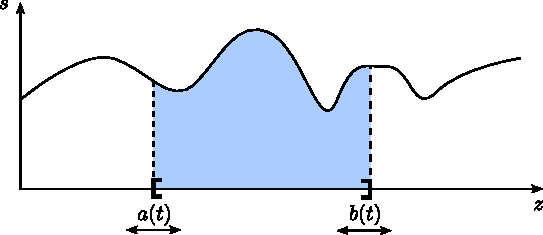
\includegraphics{img/bilanz1d}
	\label{fig:bilanz1d}
\end{figure}
\begin{itemize}
\item Wert der Bilanzgröße durch Integration über das mitbewegte Intervall $V_t=[a(t),b(t)]$
\end{itemize}
\begin{align*}
S_{V_t}=\int_{a(t)}^{b(t)}s(z,t)\d z
\end{align*}
Ableitung der Grenzen:
\begin{align*}
\frac{\partial a(t)}{\partial t} = v(a(t),t) \qquad \frac{\partial b(t)}{\partial t} = v(b(t),t)
\end{align*}
statt Anwendung des Transportsatzes von Reynolds
\begin{align*}
\frac{\d}{\d t}S_{V_t} = \frac{\d}{\d t}\int_{a(t)}^{b(t)}s(z,t)\d z &= s(b(t),t)\dot{b}(t)-s(a(t),t)\dot{a}(t)+\int_{a(t)}^{b(t)}\frac{\partial s(z,t)}{\partial t}\d z \\
&= s(b(t),t)v(b(t),t)-s(a(t),t)v(a(t),t)+\int_{a(t)}^{b(t)}\frac{\partial s(z,t)}{\partial t}\d z \\
&=\int_{a(t)}^{b(t)}\frac{\partial}{\partial z}v(z,t)s(z,t)\frac{\partial s(z,t)}{\partial t}\d z 
\end{align*}
mit der Notation aus \ref{sec:modortsfest} ergibt sich:
\begin{align}
\frac{\partial s(z,t)}{\partial t}-p(z,t)+\frac{\partial}{\partial z}(v(z,t)s(z,t)+q(z,t))= 0
\end{align}